
\documentclass[9pt]{beamer}

\usepackage[latin1]{inputenc}
\usepackage{colortbl}
\usepackage[english]{babel}

\newcommand{\myblue} [1] {{\color{blue}#1}}
\newcommand{\newauthor}[4]{
  \parbox{0.26\textwidth}{
    \texorpdfstring
      {
        \centering
        #1 \\
        \myblue{{\href{#2}{\texttt{#3}}}} \\
        #4 \\
      }
      {#1}
  }
}



% beamer template
\beamertemplatetransparentcovereddynamic
\usetheme{default}

\hypersetup{%
  pdftitle={Face detection in Go and Webassembly},%
   pdfauthor={Endre Simo},%
%
}

\title[Face detection in Go and Webassembly]{Face detection in Go and Webassembly}
\author[Endre Simo]{
 \parbox{0.26\textwidth}{
	\texorpdfstring
	  {
		\centering
 		Endre Simo \\
 		\myblue{\href{https://esimov.com}{\texttt{https://esimov.com}}} \\
 		\myblue{\href{https://github.com/esimov}{\texttt{https://github.com/esimov}}} \\
 		\myblue{\href{https://twitter/simo_endre}{\texttt{https://twitter/simo\_endre}}} \\
 	  }
	{Endre Simo}
}
 }



\begin{document}

\frame{\titlepage
}

\part<presentation>{Main Talk}

\section[slides]{slides}

\begin{frame}[fragile]
\frametitle{About me}


\end{frame}

\begin{frame}[fragile]
\frametitle{I am ...}


\begin{itemize}
\item Software developer and open source enthusiast, tackling with image processing, computer vision, machine learning and procedural graphics as side projects
\item I like the clean and readable code
\item Performance and code optimization addict
\item I consider the concurrency communication model (CSP) the most appealing parts of the Go language
\end{itemize}


\end{frame}

\begin{frame}[fragile]
\frametitle{Agenda}


\begin{itemize}
\item What is Pigo?
\item Key features
\item Technical overview
\item Pigo and GoCV (OpenCV) comparision
\item Pupils/eyes localization
\item Facial landmark points detection
\item Use cases and integrations
\item Pigo as a shared library
\item Porting Pigo to Webassembly (WASM)
\item Demo time
\item What's next?
\end{itemize}


\end{frame}

\begin{frame}[fragile]
\frametitle{What is Pigo?}


\end{frame}

\begin{frame}[fragile]
\frametitle{What is Pigo?}


\begin{figure}[h]
\begin{center}

\includegraphics[width=3cm,height=4cm]{assets/pigo_logo.png}
\end{center}

\end{figure}

\begin{itemize}
\item Computer vision and machine learning library for face detection, pupils/eyes localization and facial landmark points detection
\item The only face detection library in the Go ecosystem developed 100\% in Go
\item The implementation is based on \emph{Pixel} \emph{Intensity} \emph{Comparison-based} \emph{Object} \emph{detection} paper
\end{itemize}


\end{frame}

\begin{frame}[fragile]
\frametitle{Why it has been developed?}


\begin{itemize}
\item All of the existing face detection libraries developed in Go are actually bindings (wrappers) around some C/C++ libraries
\item Bindings (using the cgo) most of the times are not cost effective
\item Compiling a C library to Go results in slower build times
\item Cross compilation is almost impossible
\item The desire of a single binary file is just a desire
\item Installing OpenCV sometimes can be daunting
\item OpenCV is huge, impossible to deploy it on small platforms where space constraints are important
\end{itemize}


\end{frame}

\begin{frame}[fragile]
\frametitle{Key features}


What are the benefits of using Pigo over other existing solutions? Just to name a few of them:


\begin{itemize}
\item Very lightweight, no requirements for 3rd party modules and external libraries
\item Platform independent, one single executable
\item Simple and elegant API
\item High processing speed
\item There is no need for image preprocessing prior detection
\item The face detection is based on pixel intensity comparison encoded in the binary file tree structure
\item Fast detection of in-plane rotated faces
\item Pupils/eyes localization
\item Facial landmark points detection
\end{itemize}


\end{frame}

\begin{frame}[fragile]
\frametitle{Technical overview}


\end{frame}

\begin{frame}[fragile]
\frametitle{Technical overview}


\begin{itemize}
\item \textbf{Pigo}, like the \textbf{Viola} \textbf{Jones} face detection algorithm is also constructed around cascade decision trees, but the cascade classifier is in binary format
\item The role of a classifier is to tell if a face is present in the current region or not
\item The classifier consists of a decision tree, where the results of pixel intensity comparison test are in binary format.
\item Because the cascades are encoded into a binary tree structure they first need to be unpacked.
\end{itemize}


\end{frame}

\begin{frame}[fragile]
\frametitle{Upacking steps}


\begin{itemize}
\item Read the depth of each tree and write it into the buffer array.
\item Retrieve the number of stages and write it into the buffer array.
\item Obtain the scale multiplier (applied after each stage) and write it into the buffer array.
\item Obtain the number of trees per stage and write it into the buffer array.
\item Obtain the depth of each tree and write it into the buffer array.
\item Traverse all the stages of the binary tree
\item Read prediction from tree's leaf nodes.
\end{itemize}


\end{frame}

\begin{frame}[fragile]
\frametitle{Unpacking the result}


In the end we should get a cascade with the following structure:



\begin{verbatim}
return &PuplocCascade{
    stages:    stages,
    scales:    scales,
    trees:     trees,
    treeDepth: treeDepth,
    treeCodes: treeCodes,
    treePreds: treePreds,
}, nil

\end{verbatim}



\end{frame}

\begin{frame}[fragile]
\frametitle{Classify regions}


Next we classify the regions based on the parsed binary data.


For classification we are using a simple pixel intensity comparision test in binary format.



\begin{verbatim}
bintest := func(px1, px2 uint8) int {
    if px1 <= px2 {
        return 1
    }
    return 0
}
idx = 2*idx + bintest(pixels[x1], pixels[x2])

\end{verbatim}


The \texttt{idx} will be the index in the prediction tree.


\emph{Note}: for in plane rotated faces we are applying the same formula only that we are calculating the rotation angle.



\end{frame}

\begin{frame}[fragile]
\frametitle{Run cascade}


\begin{itemize}
\item An image region is considered being face if it passes all the cascade members. Since this process is limited to a relatively small number of regions, this gains high computation speed.
\item During the decision tree scanning each detection is flagged with a detection score.
\item An image region is considered as face if the detection score is above a certain threshold (\textbf{$\sim$0.995})
\item The detector function will return a struct with the following structure
\end{itemize}


\begin{verbatim}
// Detection struct contains the detection results composed of
// the row, column, scale factor and the detection score.
type Detection struct {
    Row   int
    Col   int
    Scale int
    Q     float32
}

\end{verbatim}



\end{frame}

\begin{frame}[fragile]
\frametitle{Cluster detection}


\begin{itemize}
\item Due to the noisiness of the underlying pixel data, the detector might produce overlaps in detections.
\end{itemize}

\begin{figure}[h]
\begin{center}
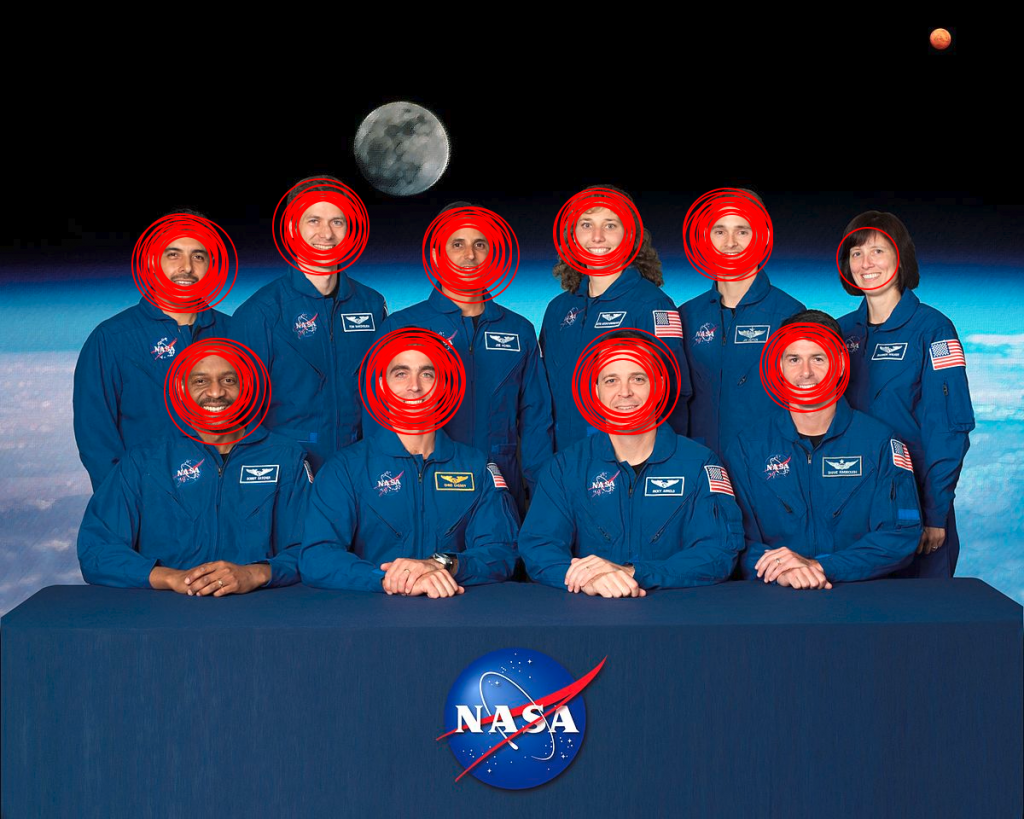
\includegraphics[width=5cm,height=4cm]{assets/pigo_output_without_clustering-1024x819.png}
\end{center}

\end{figure}

\begin{itemize}
\item The cascade regions are clustered together by aplying an \textbf{IoU} (Intersection over Union) formula over the detection results.
\end{itemize}


\end{frame}

\begin{frame}[fragile]
\frametitle{The intersection over union method}



\begin{verbatim}
sort.Sort(det(detections))

calcIoU := func(det1, det2 Detection) float64 {
    // Unpack the position and size of each detection.
    r1, c1, s1 := float64(det1.Row), float64(det1.Col), float64(det1.Scale)
    r2, c2, s2 := float64(det2.Row), float64(det2.Col), float64(det2.Scale)

    overRow := math.Max(0, math.Min(r1+s1/2, r2+s2/2)-math.Max(r1-s1/2, r2-s2/2))
    overCol := math.Max(0, math.Min(c1+s1/2, c2+s2/2)-math.Max(c1-s1/2, c2-s2/2))

    // Return intersection over union.
    return overRow * overCol / (s1*s1 + s2*s2 - overRow*overCol)
}

\end{verbatim}



\end{frame}

\begin{frame}[fragile]
\frametitle{API usage}


\begin{itemize}
\item Simple and elegant API
\item Easy integration, cross platform interoperability
\item Posibility to export the detection results to a JSON file
\item Pipeline support
\end{itemize}


\begin{verbatim}
// Initialize the cascade parameters
cParams := pigo.CascadeParams{
    MinSize:     20,
    MaxSize:     1000,
    ShiftFactor: 0.1,
    ScaleFactor: 1.1,

    ImageParams: pigo.ImageParams{
        Pixels: pixels,
        Rows:   rows,
        Cols:   cols,
        Dim:    cols,
    },
}

\end{verbatim}



\end{frame}

\begin{frame}[fragile]
\frametitle{API usage}



\begin{verbatim}
pigo := pigo.NewPigo()
// Unpack the binary file. This will return the number of cascade trees,
// the tree depth, the threshold and the prediction from tree's leaf nodes.
classifier, err := pigo.Unpack(cascadeFile)
if err != nil {
    log.Fatalf("Error reading the cascade file: %s", err)
}

angle := 0.0 // cascade rotation angle. 0.0 is 0 radians and 1.0 is 2*pi radians

// Run the classifier over the obtained leaf nodes and return the detection results.
// The result contains quadruplets representing the row, column, scale and detection score.
dets := classifier.RunCascade(cParams, angle)

// Calculate the intersection over union (IoU) of two clusters.
dets = classifier.ClusterDetections(dets, 0.2)

\end{verbatim}


\begin{itemize}
\item dets will return the coordinates of the detected faces, eyes and landmark points depending on the provided parameters
\end{itemize}


\begin{verbatim}
{"face":{"x":422,"y":336,"size":483},"eyes":[{"x":378,"y":267,"size":39},{"x":380,"y":432,"size":40}]}

\end{verbatim}



\end{frame}

\begin{frame}[fragile]
\frametitle{End result}


\begin{figure}[h]
\begin{center}
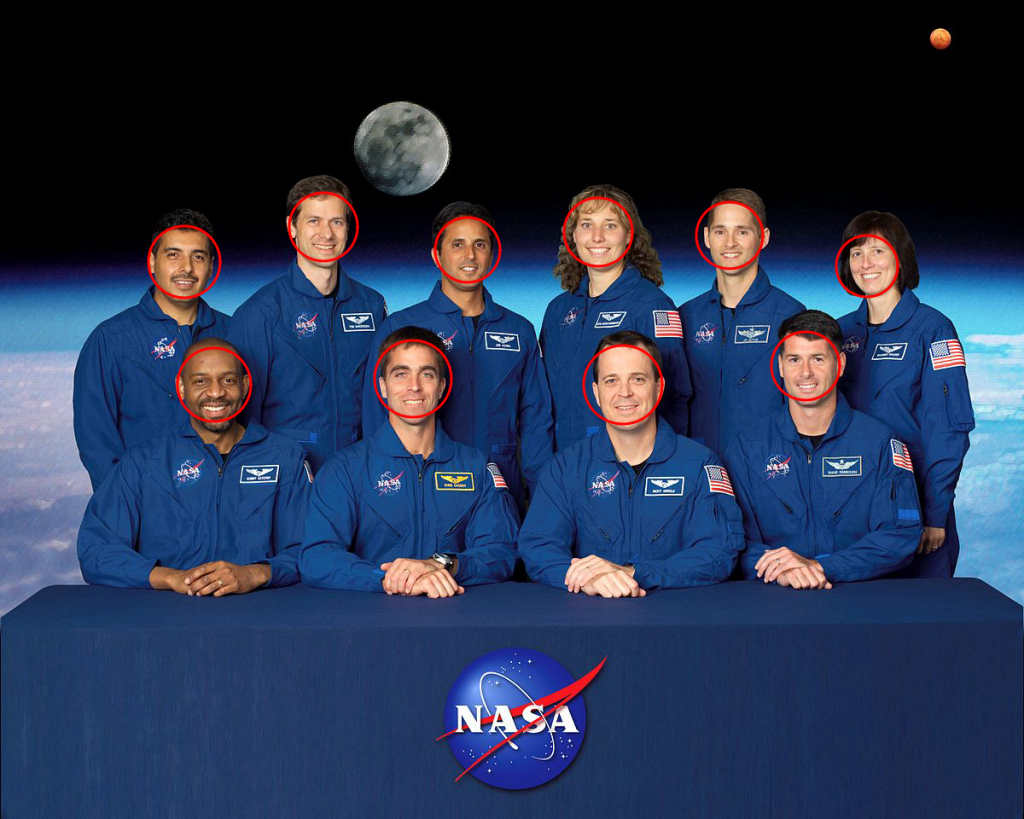
\includegraphics[width=9cm,height=7cm]{assets/pigo_clustering-1024x819.png}
\end{center}

\end{figure}


\end{frame}

\begin{frame}[fragile]
\frametitle{Pigo and GoCV (OpenCV) comparision}


\end{frame}

\begin{frame}[fragile]
\frametitle{Benchmark results}



\begin{verbatim}
BenchmarkGoCV-4              3     414122553 ns/op         704 B/op           1 allocs/op
BenchmarkPIGO-4             10     173664832 ns/op           0 B/op           0 allocs/op
PASS
ok      github.com/esimov/gocv-test    4.530s

\end{verbatim}


\myblue{\href{https://github.com/esimov/pigo-gocv-benchmark}{\texttt{github.com/esimov/pigo-gocv-benchmark}}}


\end{frame}

\begin{frame}[fragile]
\frametitle{Pupils/eyes localization}


\end{frame}

\begin{frame}[fragile]
\frametitle{Pupils/eyes localization}


\begin{figure}[h]
\begin{center}
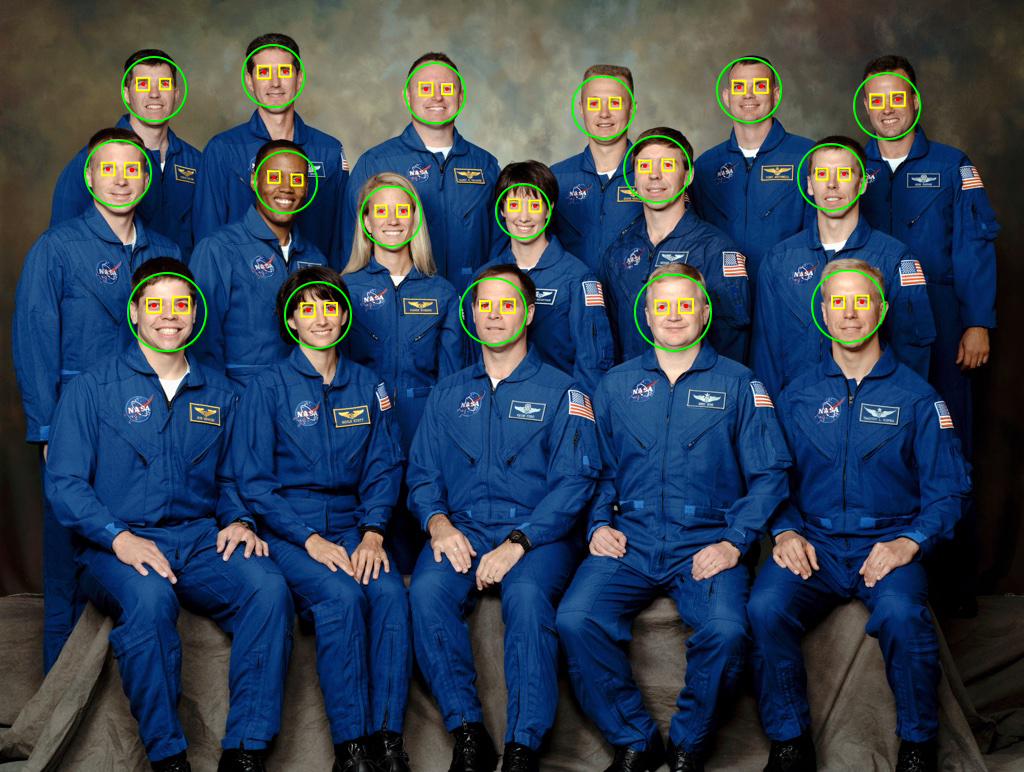
\includegraphics[width=10cm,height=7cm]{assets/pigo_puploc.png}
\end{center}

\end{figure}


\end{frame}

\begin{frame}[fragile]
\frametitle{Short overview}


\begin{itemize}
\item The implementation pretty much resambles with the face detection method but with few remarkable differences.
\end{itemize}

\begin{itemize}
\item As on the face detection, the detection is based on the same pixel intensity binary test.
\item The output of the regression trees might be noisy
\item We introduce a random perturbation factor during runtime to outweigh the false positive rates on detection
\end{itemize}

\begin{figure}[h]
\begin{center}
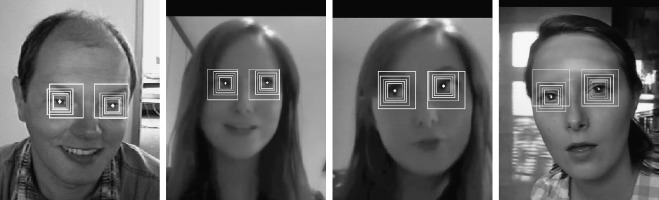
\includegraphics[width=7cm,height=2cm]{assets/puploc_perturbation.jpg}
\end{center}

\end{figure}

\begin{itemize}
\item After the face region has been classified we sort the perturbations in ascendant order.
\end{itemize}


\end{frame}

\begin{frame}[fragile]
\frametitle{Left/right face detection}


Same formula for left and rigth eye detection. The sign is flipped on the right eye.



\begin{verbatim}
// left eye
puploc = &pigo.Puploc{
    Row:      face.Row - int(0.075*float32(face.Scale)),
    Col:      face.Col - int(0.175*float32(face.Scale)),
    Scale:    float32(face.Scale) * 0.25,
    Perturbs: perturb,
}

// right eye
puploc = &pigo.Puploc{
    Row:      face.Row - int(0.075*float32(face.Scale)),
    Col:      face.Col + int(0.185*float32(face.Scale)),
    Scale:    float32(face.Scale) * 0.25,
    Perturbs: perturb,
}

\end{verbatim}



\end{frame}

\begin{frame}[fragile]
\frametitle{Facial landmark points detection}


\end{frame}

\begin{frame}[fragile]
\frametitle{Facial landmark points detection}


\begin{figure}[h]
\begin{center}
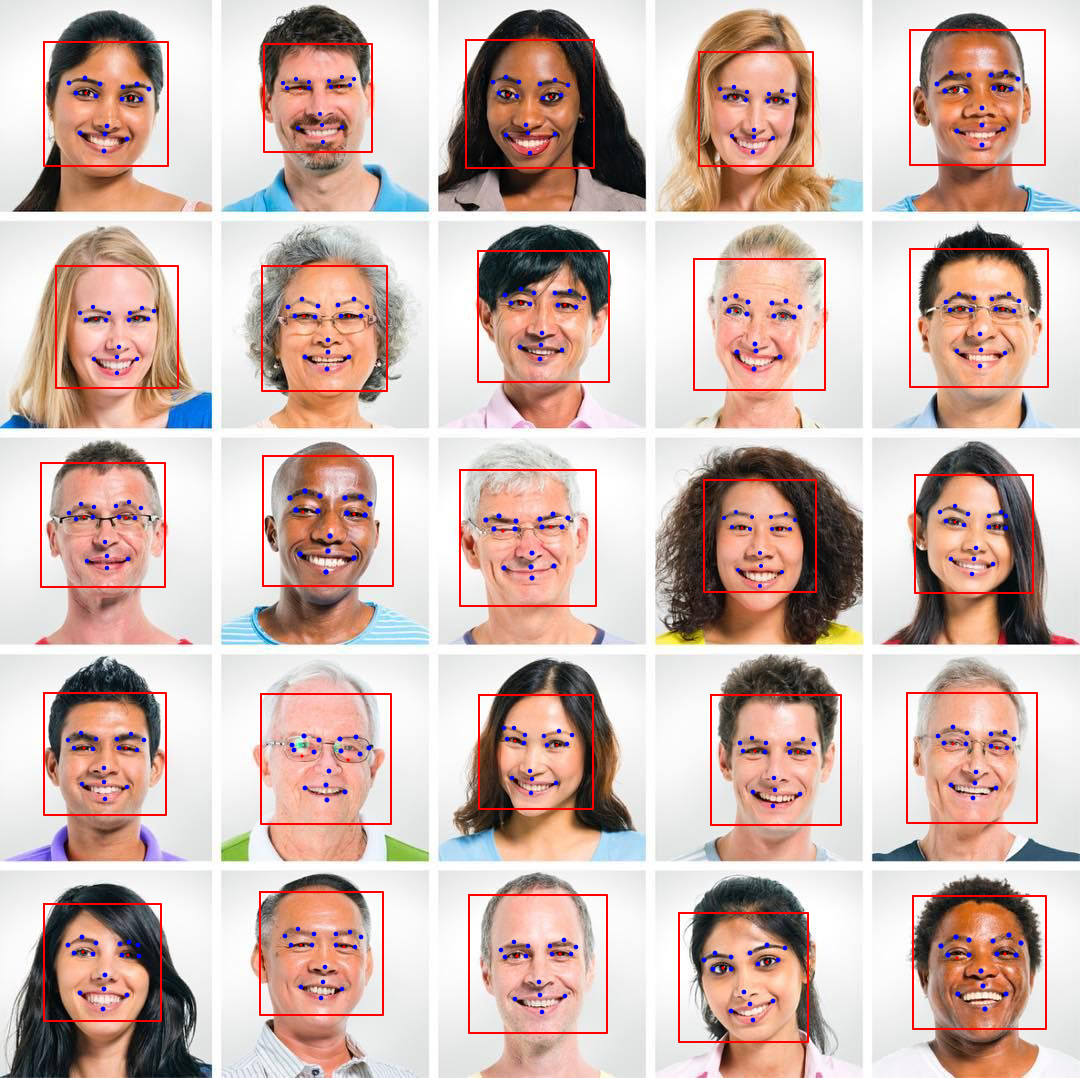
\includegraphics[width=7cm,height=7cm]{assets/pigo_landmark.png}
\end{center}

\end{figure}


\end{frame}

\begin{frame}[fragile]
\frametitle{Detection method}


\begin{itemize}
\item The landmark points are detected based on the results returned by the pupil localization function
\end{itemize}


\begin{verbatim}
dist1 := (leftEye.Row - rightEye.Row) * (leftEye.Row - rightEye.Row)
dist2 := (leftEye.Col - rightEye.Col) * (leftEye.Col - rightEye.Col)
dist := math.Sqrt(float64(dist1 + dist2))

row := float64(leftEye.Row+rightEye.Row)/2.0 + 0.25*dist
col := float64(leftEye.Col+rightEye.Col)/2.0 + 0.15*dist
scale := 3.0 * dist

flploc = &Puploc{
    Row:      int(row),
    Col:      int(col),
    Scale:    float32(scale),
    Perturbs: perturb,
}

\end{verbatim}



\end{frame}

\begin{frame}[fragile]
\frametitle{Compute the right landmark points}


This can be achieved by:


1.) flipping the sign of the column coordinate in tree nodes



\begin{verbatim}
if flipV {
    c1 = min(ncols-1, max(0, (256*int(c)+int(-plc.treeCodes[root+4*idx+1])*int(round(float64(s))))>>8))
    c2 = min(ncols-1, max(0, (256*int(c)+int(-plc.treeCodes[root+4*idx+3])*int(round(float64(s))))>>8))
} else {
    c1 = min(ncols-1, max(0, (256*int(c)+int(plc.treeCodes[root+4*idx+1])*int(round(float64(s))))>>8))
    c2 = min(ncols-1, max(0, (256*int(c)+int(plc.treeCodes[root+4*idx+3])*int(round(float64(s))))>>8))
}

\end{verbatim}


2.) flipping the sign in the column coordinate for each binary test



\begin{verbatim}
if flipV {
    dc += -plc.treePreds[lutIdx+1]
} else {
    dc += plc.treePreds[lutIdx+1]
}

\end{verbatim}



\end{frame}

\begin{frame}[fragile]
\frametitle{Use cases and integrations}


\end{frame}

\begin{frame}[fragile]
\frametitle{OpenFaaS integration}


\begin{figure}[h]
\begin{center}
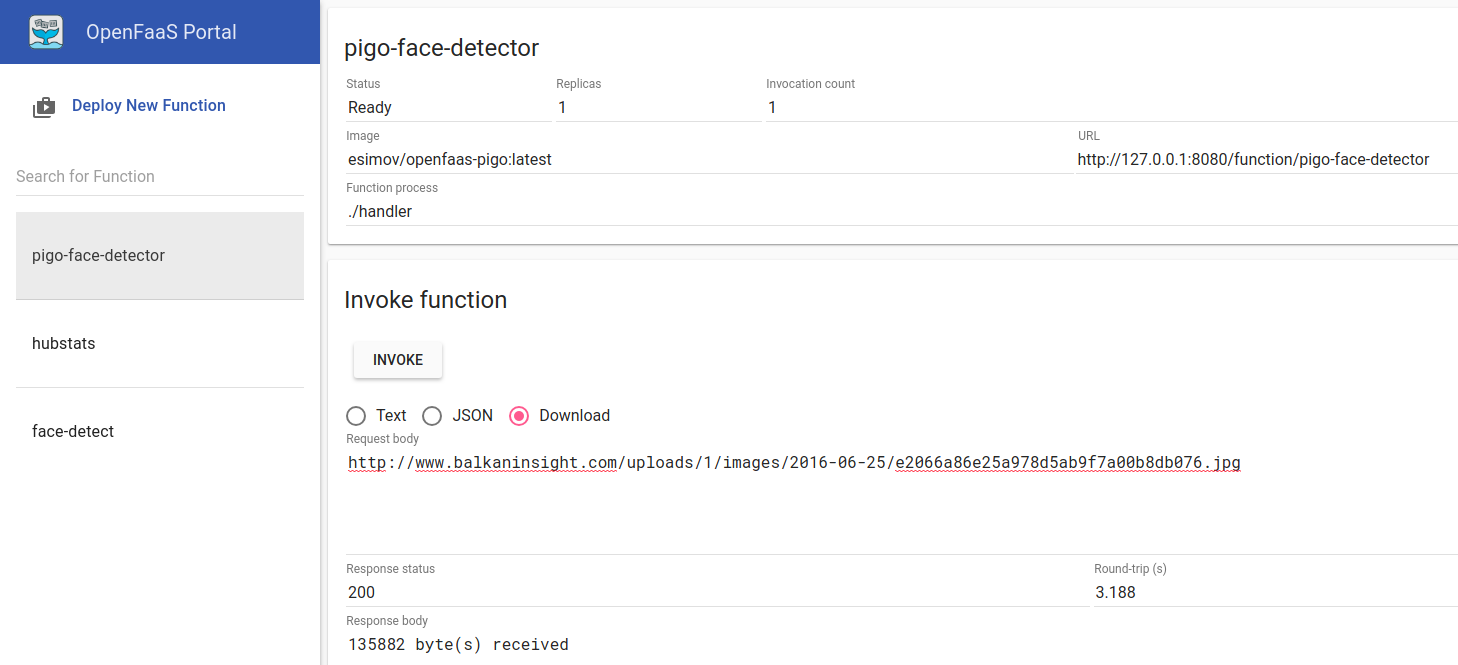
\includegraphics[width=10cm,height=4cm]{assets/pigo_openfaas.png}
\end{center}

\end{figure}


\end{frame}

\begin{frame}[fragile]
\frametitle{OpenFaaS integration}


\begin{figure}[h]
\begin{center}
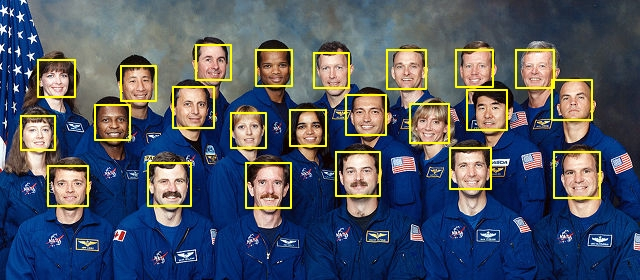
\includegraphics[width=9cm,height=4cm]{assets/pigo_openfaas_result.jpg}
\end{center}

\end{figure}

\myblue{\href{https://github.com/esimov/pigo-openfaas}{\texttt{github.com/esimov/pigo-openfaas}}}


\end{frame}

\begin{frame}[fragile]
\frametitle{OpenFaaS intergation}


\begin{figure}[h]
\begin{center}
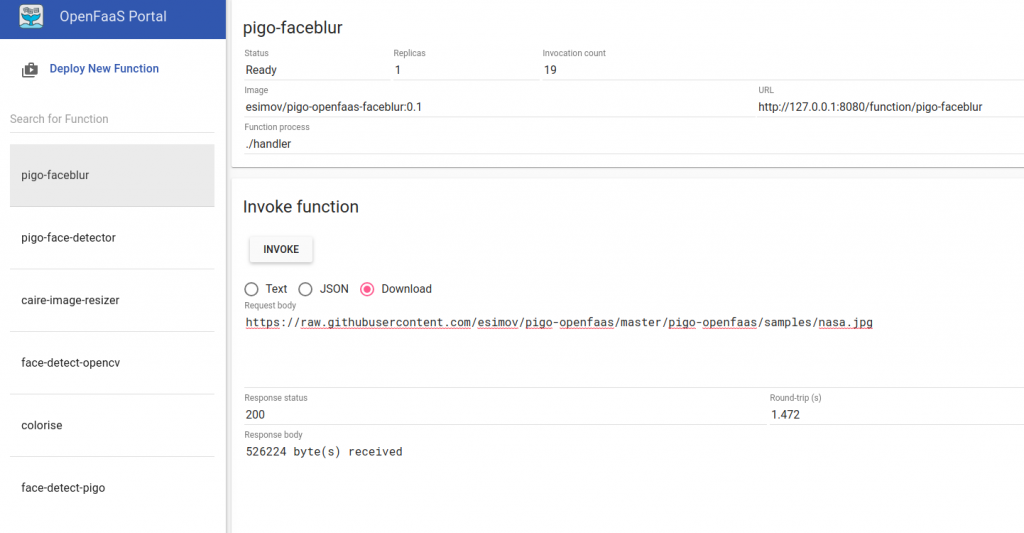
\includegraphics[width=9cm,height=4cm]{assets/pigo_openfaas-blur.png}
\end{center}

\end{figure}


\end{frame}

\begin{frame}[fragile]
\frametitle{OpenFaaS integration}


\begin{figure}[h]
\begin{center}
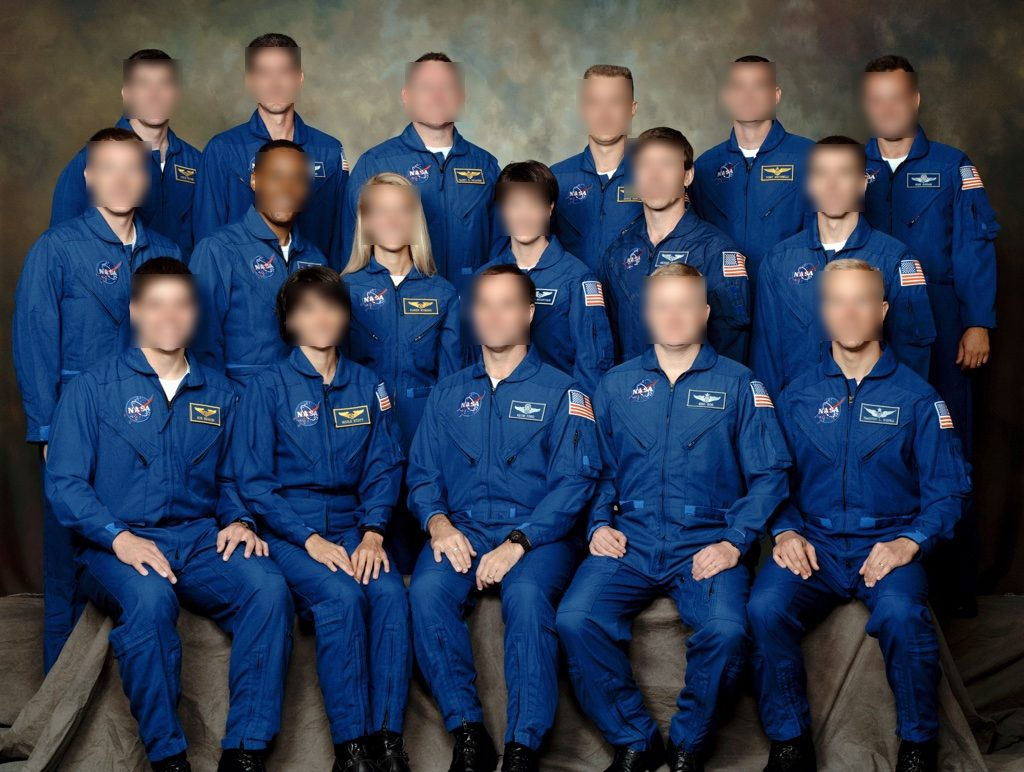
\includegraphics[width=7cm,height=5cm]{assets/pigo_openfaas-blur_result.jpg}
\end{center}

\end{figure}

\myblue{\href{https://github.com/esimov/pigo-openfaas-faceblur}{\texttt{github.com/esimov/pigo-openfaas-faceblur}}}

\myblue{\href{https://github.com/esimov/stackblur-go}{\texttt{github.com/esimov/stackblur-go}}}


\end{frame}

\begin{frame}[fragile]
\frametitle{Other integration}


\begin{figure}[h]
\begin{center}
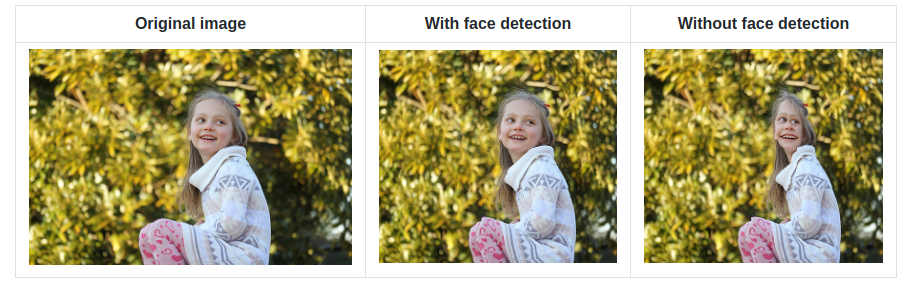
\includegraphics[width=12cm,height=4cm]{assets/caire-example.png}
\end{center}

\end{figure}

Avoiding face deformation in Caire


\myblue{\href{https://github.com/esimov/caire}{\texttt{github.com/esimov/caire}}}


\end{frame}

\begin{frame}[fragile]
\frametitle{Pigo as a shared library}


\end{frame}

\begin{frame}[fragile]
\frametitle{Running the face detector from Python as shared library}


\begin{itemize}
\item Go is missing a well founded and generally available webcam library
\end{itemize}

\begin{itemize}
\item The idea is to transfer the Go face detection results to Python as a shared object (\texttt{.so}) library
\item A few things we need to take care:
\end{itemize}


\begin{verbatim}
The exported function should be annotated with the //export statement.
The source must import the pseudo C package.
An empty main function should be declared.
The package must be a main package.

\end{verbatim}


\begin{itemize}
\item In Python the \textbf{Ctype} library is used to interoperate with the Go code through \textbf{cgo}
\item It provides C compatible data types, and allows calling functions in DLLs or shared libraries.
\end{itemize}


\end{frame}

\begin{frame}[fragile]
\frametitle{Limitations}


\begin{itemize}
\item In Go is not possible transfer a 2D array as an array pointer.
\item The trick is to convert the 2D array to a 1D array.
\end{itemize}


\begin{verbatim}
|-> delimit each detection group
|-> introduce as a first slice element the number of detected faces

\end{verbatim}


\begin{itemize}
\item Using the \textbf{numpy} library we transform it to the desired shape.
\item In the end we should obtain something like below:
\end{itemize}


\begin{verbatim}
[2 0 0 0 0 272 297 213 41 1 248 258 27 41 0 248 341 27 41 0 238 599 72 25 1 230 587 9 25 0 233 616 9 25 0]

\end{verbatim}


where the first value represents the number of detected faces and the rest are the \textbf{x}, \textbf{y} position and the \textbf{scale} factor



\end{frame}

\begin{frame}[fragile]
\frametitle{Transfer the detection result from Go to Python}



\begin{verbatim}
go func() {
    // Since in Go we cannot transfer a 2d array trough an array pointer
    // we have to transform it into 1d array.
    for _, v := range result {
        det = append(det, v...)
    }
    // Include as a first slice element the number of detected faces.
    // We need to transfer this value in order to define the Python array buffer length.
    det = append([]int{len(result), 0, 0}, det...)

    // Convert the slice into an array pointer.
    s := *(*[]uint8)(unsafe.Pointer(&det))
    p := uintptr(unsafe.Pointer(&s[0]))

    // Ensure `det` is not freed up by GC prematurely.
    runtime.KeepAlive(det)

    // return the pointer address
    pointCh <- p
}()
return <-pointCh

\end{verbatim}



\end{frame}

\begin{frame}[fragile]
\frametitle{Some caveats}


\begin{itemize}
\item The cost using cgo can be substantial
\item C and Go exists in two different universe, they interoperate through cgo. This is not costs effective.
\item The C compiler has to be invoked for every C file in the package.
\item Slower build times
\item Ctype introduce another latency factor
\end{itemize}


\end{frame}

\begin{frame}[fragile]
\frametitle{Porting Pigo to Webassembly (WASM)}


\end{frame}

\begin{frame}[fragile]
\frametitle{Pigo and Webassembly}


\end{frame}

\begin{frame}[fragile]
\frametitle{Motivation}


\begin{itemize}
\item Running Pigo in Python as shared object does not showed the library pure performance
\item Webassembly is an emerging technology targeting the web browser and bringing almost native like performance
\item Many low level languages are already offer support for WASM (C, C++, Rust, Go etc.)
\item More and more projects are getting ported to WASM
\item Go already offer good Webassembly support trough the \textbf{syscall/js} package
\item Go \textbf{v1.11} was the first version targeting WASM
\item The API has gone through some refactorings and improvements to be stable starting from \textbf{v1.13}
\end{itemize}


\end{frame}

\begin{frame}[fragile]
\frametitle{Considerations to keep in mind}


\begin{itemize}
\item To access a Javascript global variable in Go you have to call the \textbf{js.Global()} function.
\item Use the \textbf{Call()} function in Go in order to call a JS method.
\item To get or set an attribute of a JS object or Html element we can call the \textbf{Get()} or \textbf{Set()} functions.
\item \emph{The} \emph{JavaScript} \emph{callback} \emph{functions} \emph{should} \emph{always} \emph{be} \emph{invoked} \emph{inside} \emph{a} \emph{goroutine ,} \emph{otherwise} \emph{you} \emph{will} \emph{encounter} \emph{deadlock}
\item The JS methods need to be used for fetching a file. The standard \textbf{io} package is not usable here.
\item In order to compile for Webassambly we need to explicitly specify and set the \textbf{GOOS=js} and \textbf{GOARCH=wasm} environment variables on the building process
\end{itemize}


\begin{verbatim}
$ GOOS=js GOARCH=wasm go build -o lib.wasm wasm.go

\end{verbatim}



\end{frame}

\begin{frame}[fragile]
\frametitle{Building the wasm file}


We need to use the following build constraint



\begin{verbatim}
// +build js,wasm*

\end{verbatim}


The \textbf{Render()} method will call the underlying JS render method:



\begin{verbatim}
// +build js,wasm

package main

import (
    "github.com/esimov/pigo/wasm/canvas"
)

func main() {
    c := canvas.NewCanvas()
    webcam, err := c.StartWebcam()
    if err != nil {
        c.Alert("Webcam not detected!")
    } else {
        webcam.Render()
    }
}

\end{verbatim}



\end{frame}

\begin{frame}[fragile]
\frametitle{The Render() method:}



\begin{verbatim}
func (c *Canvas) Render() {
    var data = make([]byte, c.windowSize.width*c.windowSize.height*4)
    c.done = make(chan struct{})

    if err := det.UnpackCascades(); err == nil {
        c.renderer = js.FuncOf(func(this js.Value, args []js.Value) interface{} {
            go func() {
                width, height := c.windowSize.width, c.windowSize.height
                c.reqID = c.window.Call("requestAnimationFrame", c.renderer)
                c.ctx.Call("drawImage", c.video, 0, 0)
                rgba := c.ctx.Call("getImageData", 0, 0, width, height).Get("data")

                uint8Arr := js.Global().Get("Uint8Array").New(rgba)
                js.CopyBytesToGo(data, uint8Arr)
                pixels := c.rgbaToGrayscale(data)
                res := det.DetectFaces(pixels, height, width)
                c.drawDetection(res)
            }()
            return nil
        })
        c.window.Call("requestAnimationFrame", c.renderer)
        <-c.done
    }
}

\end{verbatim}



\end{frame}

\begin{frame}[fragile]
\frametitle{Calling the WASM file}


The WASM file can be referenced in the main html file.



\begin{verbatim}
<script type="text/javascript">
    function fetchAndInstantiate(url, importObject) {
        return fetch(url).then(response =>
            response.arrayBuffer()
        ).then(bytes =>
            WebAssembly.instantiate(bytes, importObject)
        ).then(results =>
            results.instance
        );
    }
    var go = new Go();
    var mod = fetchAndInstantiate("lib.wasm", go.importObject);
    window.onload = function () {
        mod.then(function (instance) {
            go.run(instance);
        });
    };
</script>

\end{verbatim}



\end{frame}

\begin{frame}[fragile]
\frametitle{wasm\_exec.js}


\begin{itemize}
\item Incompatibilities between Go versions
\item Different Go versions have different \textbf{wasm\_exec.js} file
\item Copy the wasm\_exec.js file from \textbf{\$GOROOT} on the fly.
\end{itemize}


\begin{verbatim}
wasm:
    cp -f "$$(go env GOROOT)/misc/wasm/wasm_exec.js" ./js/
    GOOS=js GOARCH=wasm go build -o lib.wasm wasm.go

\end{verbatim}



\end{frame}

\begin{frame}[fragile]
\frametitle{Demo time}


\begin{itemize}
\item New repository exists to showcase WASM demos using the Pigo libray (this is continuously updated)
\end{itemize}

\myblue{\href{https://github.com/esimov/pigo-wasm-demos}{\texttt{github.com/esimov/pigo-wasm-demos}}}


\end{frame}

\begin{frame}[fragile]
\frametitle{What's next?}


\begin{itemize}
\item Image features detection and matching (to detect similarities inside images)
\item Possible features detection methods: SIFT, SURF (faster)
\item This can be a starting point for facial recognition
\end{itemize}


\end{frame}

\end{document}
